\documentclass[11pt]{article}
\usepackage[margin=1in]{geometry}
\usepackage{graphicx}
\usepackage{booktabs}
\usepackage{xcolor}
\usepackage{hyperref}
\usepackage{amsmath}
\usepackage{listings}
\usepackage{enumitem}
\usepackage{caption}
\usepackage{float}
\usepackage{longtable}

\hypersetup{colorlinks=true, linkcolor=blue, urlcolor=blue, citecolor=blue}

\definecolor{codebg}{rgb}{0.96,0.96,0.96}
\lstset{
  basicstyle=\ttfamily\small,
  backgroundcolor=\color{codebg},
  frame=single,
  breaklines=true,
  columns=fullflexible,
  keywordstyle=\color{blue!70!black}\bfseries,
  commentstyle=\color{green!40!black}\itshape,
  stringstyle=\color{orange!70!black},
  language=C++,
  tabsize=2,
}

\title{\Large\textbf{Lab Assignment Report: Multiple Access ---\\ CDMA with Walsh Codes}}
\author{Sajjad Ahmed Shaaz \\ 002410501093 \\ BCSE-III A3}
\date{November 2, 2026}

\begin{document}
\maketitle

\section*{Basic Information}
\begin{itemize}[leftmargin=1.6em]
  \item \textbf{Subject:} CSE/PC/B/S/314 Computer Networks Lab
  \item \textbf{Assignment Number:} 4
  \item \textbf{Problem Statement:} Implement CDMA for multiple access of a common channel
  by $n$ stations. Each sender uses a unique code word, given by the Walsh set, to encode its
  data and send it across the channel; the data must then be perfectly reconstructed at the
  $n$ receiving stations. The same sender--receiver design as the previous assignments is
  to be used.
  \item \textbf{Code demonstration due:} 05--09 October 2026 \quad
  \textbf{Report submission due:} next lab class
\end{itemize}

\section{Design}

\subsection{Purpose of the Program}
Assignment 3 shared one channel among $N$ stations by \emph{taking turns}: carrier sensing
and backoff decide who may transmit, and two stations transmitting together is a collision
that destroys both frames. CDMA (Code Division Multiple Access) removes the turn-taking
entirely. Every station transmits \emph{at the same time} on the \emph{same} channel; the
signals add up on the medium, and each receiver extracts only the station it is interested
in by correlating the sum with that station's code. With Walsh codes, which are mutually
orthogonal, every other station's contribution cancels \emph{exactly}. A ``collision'' is no
longer a failure; it is the normal operating condition.

This program implements that scheme end to end. $N$ independent sender processes spread
their data with Walsh codes, a shared channel process adds their signals chip by chip
(optionally adding noise), and $N$ independent receiver processes despread the common
signal and write their sender's file to disk byte-for-byte.

\subsection{Background: Walsh Codes and Despreading}
A Walsh code of length $L = 2^k$ is a row of the $L\times L$ Hadamard matrix built by
Sylvester's recursion:
\[
W_1 = [+1], \qquad
W_{2n} = \begin{bmatrix} W_n & W_n \\ W_n & -W_n \end{bmatrix}.
\]
Any two distinct rows are orthogonal: $c_a \cdot c_b = \sum_j c_a[j]\,c_b[j] = 0$ for $a\neq b$,
and $c_a\cdot c_a = L$ (Figure~\ref{fig:walsh}). Station $i$ maps each data bit to
$d_i\in\{+1,-1\}$ (or $d_i = 0$ when it has nothing to send) and transmits the $L$ chips
$d_i\,c_i$. The channel delivers the chip-wise sum plus noise, $S[j] = \sum_k d_k c_k[j] + n_j$,
and receiver $i$ computes
\[
v_i \;=\; \frac{1}{L}\, S\cdot c_i
\;=\; d_i \;+\; \underbrace{\frac{1}{L}\sum_{k\neq i} d_k\,(c_k\cdot c_i)}_{=\,0 \text{ for Walsh codes}}
\;+\; \underbrace{\frac{1}{L}\sum_j n_j\,c_i[j]}_{\eta_i \,\sim\, \mathcal{N}(0,\;\sigma^2/L)} .
\]
The middle term, \emph{multiple-access interference} (MAI), vanishes identically for Walsh
codes, so in a noiseless channel $v_i = d_i$ exactly. This holds regardless of how many
other stations transmit or what they send. In a noisy channel the despreading also
\emph{averages} the noise over $L$ chips, reducing its standard deviation from $\sigma$ to
$\sigma/\sqrt{L}$ (the \emph{processing gain}).

\begin{figure}[H]
\centering
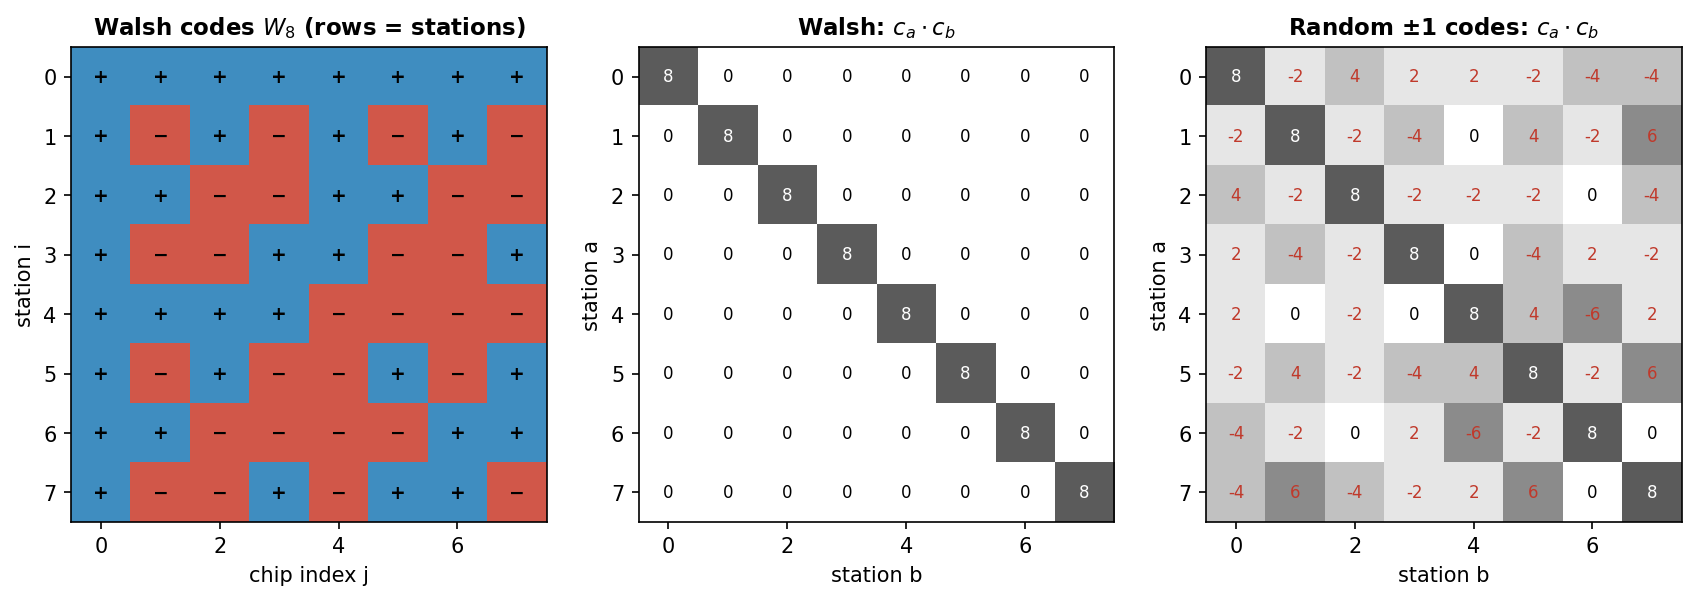
\includegraphics[width=\textwidth]{figures/walsh_codes.png}
\caption{Left: the $8\times8$ Walsh matrix produced by \texttt{walshMatrix(8)}. Middle: its
cross-correlation matrix $W W^\top = 8I$ (perfectly orthogonal). Right: the same matrix for
eight random $\pm1$ codes of length 8: the non-zero off-diagonal entries (red) are the
source of multiple-access interference.}
\label{fig:walsh}
\end{figure}

\subsection{Design Rationale}
\paragraph{Same server + independent processes design as Assignment 3.} A central
\texttt{channel\_server} emulates the shared medium, and each station is its own OS process
talking to it over TCP. The assignment asks for separate senders and receivers, so a
station is split into a \texttt{sender} (spreads its file) and a \texttt{receiver} (despreads
and reconstructs it), both registering with the same station id $i$. The receiver has no
side channel to its sender; the only thing they share is the code, and the only thing the
receiver ever sees is the summed signal of \emph{all} senders.

\paragraph{Lock-step bit-slots (chip synchronisation).} Walsh orthogonality holds only when
all senders' chips are aligned in time; a shift of even one chip destroys it. As in
Assignment 3, the channel therefore drives everyone through discrete slots in lock-step: one
slot carries one bit from every sender, i.e.\ $L$ chips. The server collects every sender's
chips for slot $k$ before forming the sum, so alignment is guaranteed. This is the
synchronous-CDMA model of a cellular downlink (e.g.\ the IS-95 forward link, where the
base station transmits all Walsh-coded channels in perfect alignment).

\paragraph{Encoding at the sender, decoding at the receiver.} The sender really transmits
the $L$ spread chips, not its bit, and the receiver gets only the summed chips. Spreading and
despreading are therefore performed where they would be in a real system, and the server
stays a ``dumb'' medium that only adds signals (and noise).

\paragraph{A third level for silence.} Stations have messages of different lengths. A
finished sender transmits all-zero chips ($d=0$), so its receiver sees $v\approx0$ and knows
no bit was sent in that slot. The receiver therefore makes a three-way decision with
thresholds at $\pm0.5$, halfway between the levels $\{-1,0,+1\}$. This lets every station
send an arbitrary-length (even empty) file with no length header.

\paragraph{An omniscient channel server for statistics.} The server knows every code and
every sender's chips, so it can recover what each sender actually transmitted
($\operatorname{sign}(x\cdot c_i)$). Each receiver reports its decoded symbol for every slot
(\texttt{DECODED}), and the server counts bit errors directly. As in Assignment 3, this
mirrors an external analyser instrumenting the medium.

\paragraph{Optional channel impairments.} Two switches turn the ideal channel into a
realistic one so the design can be stress-tested. Additive Gaussian noise of standard
deviation $\sigma$ can be added to every chip. Random (non-orthogonal) $\pm1$ codes can be
swapped in for Walsh codes as a control, isolating exactly what orthogonality buys.

\subsection{Protocol Between Channel Server, Senders and Receivers}
Table~\ref{tab:protocol} lists the messages; Figure~\ref{fig:arch} shows the structure.
TCP (reliable, ordered) is only the coordination transport for this lock-step handshake.
The modelled CDMA channel is the arithmetic sum performed by the server.

\begin{table}[H]
\centering
\begin{tabular}{llp{7.0cm}}
\toprule
\textbf{Direction} & \textbf{Message} & \textbf{Purpose} \\
\midrule
Station $\to$ Server & \texttt{REGISTER SENDER\textbar RECEIVER i} & Join as sender/receiver of station $i$ \\
Server $\to$ Station & \texttt{CODE i L c0 \ldots c(L-1)} & Station $i$'s chip sequence \\
Server $\to$ Sender & \texttt{SLOT k} & Start of bit-slot $k$ \\
Sender $\to$ Server & \texttt{CHIPS k x0 \ldots x(L-1)} & Spread bit $x = d\cdot c_i$ \\
Sender $\to$ Server & \texttt{IDLE k} & No data left (all-zero chips) \\
Server $\to$ Receiver & \texttt{SIGNAL k S0 \ldots S(L-1)} & Composite channel signal (sum + noise) \\
Receiver $\to$ Server & \texttt{DECODED k 1\textbar 0\textbar -} & Decoded symbol (\texttt{-} = sender silent) \\
Server $\to$ all & \texttt{DONE} & Every sender idle in the same slot: end of run \\
\bottomrule
\end{tabular}
\caption{Wire protocol between \texttt{channel\_server}, \texttt{sender} and \texttt{receiver}.}
\label{tab:protocol}
\end{table}

\begin{figure}[H]
\centering
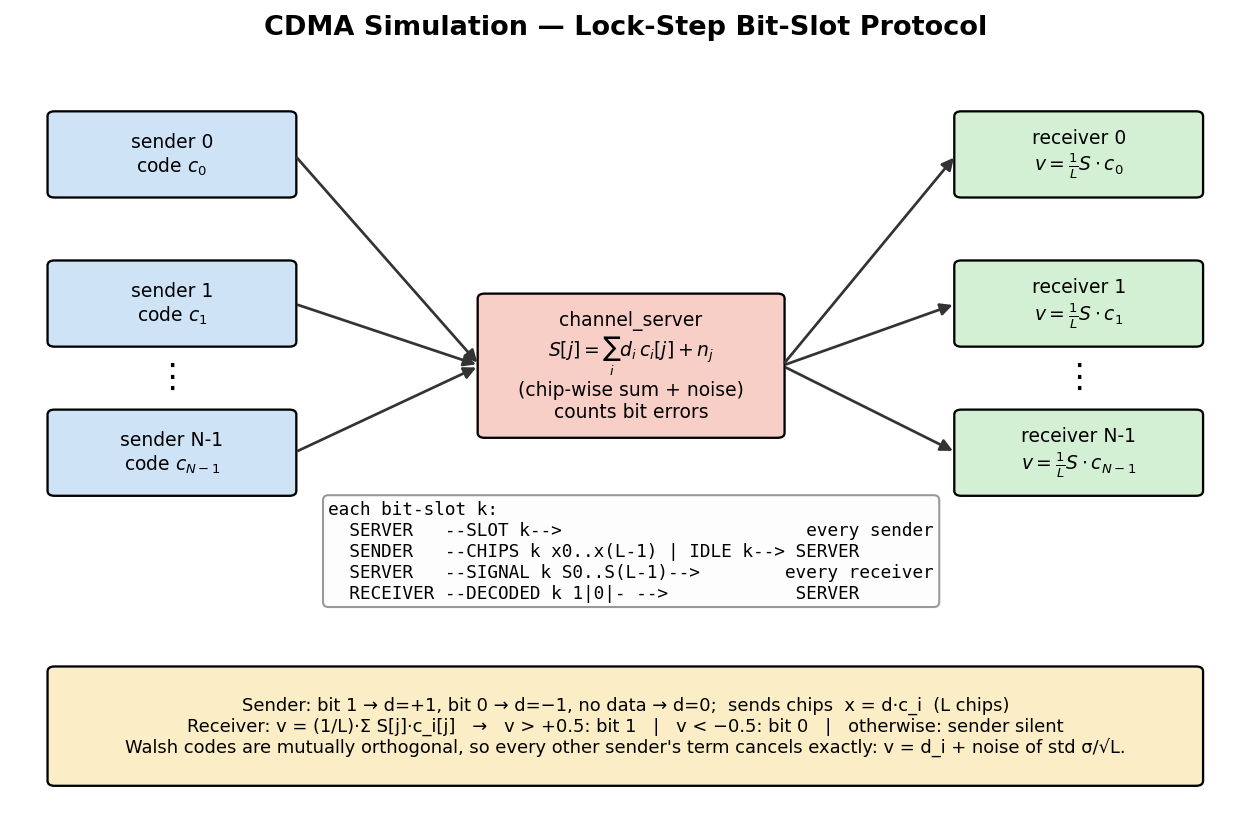
\includegraphics[width=0.95\textwidth]{figures/architecture.png}
\caption{Procedural structure: $N$ senders and $N$ receivers coordinated by the channel
server in lock-step bit-slots.}
\label{fig:arch}
\end{figure}

\subsection{Input and Output Format}
\textbf{Input:} \texttt{channel\_server} takes a port, the station count $N$, the code type
(\texttt{walsh} or \texttt{random}), the code length $L$ (0 = smallest power of two
$\ge N$), the per-chip noise $\sigma$, a random seed, and optionally a demo delay in ms. Each
\texttt{sender} takes the server address, its station id and an input file of any content
(text or binary). Each \texttt{receiver} takes the server address, its station id and an
output file path.
\textbf{Output:} each receiver writes the reconstructed file. All three programs log a
summary to \texttt{stderr}. \texttt{channel\_server} prints one CSV line to \texttt{stdout},
and in demo mode a per-slot trace (bits sent, summed signal, decoded bits), for example:
\begin{lstlisting}[language={}]
RESULT,code,N,L,sigma,slots,data_bits,bit_errors,silence_errors,ber,bits_per_chip
RESULT,walsh,4,4,0.000,40,112,0,0,0.000000,0.7000

slot    2  sent=0001  channel=[-2 -2 -2 +2 ]  decoded=0001
slot   16  sent=-00-  channel=[-2 +0 +0 +2 ]  decoded=-00-
\end{lstlisting}

\section{Implementation}
The project is implemented in C++17 with POSIX TCP sockets, plus Python scripts for the
experiment sweeps and figures.

\subsection{Component Breakdown}
\begin{itemize}[leftmargin=1.6em]
  \item \texttt{channel\_server.cpp}: the shared medium. Assigns codes, sums chips, adds
  noise, broadcasts the composite signal, and tallies bit errors.
  \item \texttt{sender.cpp}: reads a file, converts it to bits (MSB first), and spreads one
  bit per slot with its code.
  \item \texttt{receiver.cpp}: despreads the composite signal with its code, makes the
  three-level decision, packs bits into bytes, and writes the output file.
  \item \texttt{common/walsh.h}: Sylvester construction of the Walsh matrix,
  \texttt{nextPow2}, and the random-code baseline.
  \item \texttt{common/protocol.h}: message format and shared enums.
  \item \texttt{common/net\_util.h}: the buffered newline-delimited \texttt{LineSocket},
  reused unchanged from Assignment 3.
  \item \texttt{run\_experiments.py}: spawns a server and $2N$ station processes per
  configuration, parses \texttt{RESULT}, byte-compares every output file with its input,
  and writes \texttt{results/*.csv}.
  \item \texttt{report/make\_plots.py}: generates every figure in this report from the CSVs.
\end{itemize}

\subsection{Walsh Code Generation}
\begin{lstlisting}
inline vector<vector<int>> walshMatrix(int L) {      // L must be a power of 2
    vector<vector<int>> W(1, vector<int>(1, 1));    // W1 = [+1]
    for (int n = 1; n < L; n <<= 1) {
        vector<vector<int>> next(2 * n, vector<int>(2 * n));
        for (int r = 0; r < n; r++)
            for (int c = 0; c < n; c++) {
                next[r][c]         =  W[r][c];      // [ W  W ]
                next[r][c + n]     =  W[r][c];      // [ W -W ]
                next[r + n][c]     =  W[r][c];
                next[r + n][c + n] = -W[r][c];
            }
        W = next;
    }
    return W;
}
\end{lstlisting}
Station $i$ is given row $i$ of $W_L$ with $L = 2^{\lceil\log_2 N\rceil}$. The server
refuses a Walsh configuration whose $L$ is not a power of two or is smaller than $N$, since
there would not be enough orthogonal rows.

\subsection{Spreading (Sender)}
\begin{lstlisting}
int bit = (data[sentBits / 8] >> (7 - sentBits % 8)) & 1;   // MSB first
int d = bit ? 1 : -1;                                       // bit 1 -> +1, bit 0 -> -1
string msg = "CHIPS " + to_string(k);
for (int c : code) msg += (d * c > 0) ? " 1" : " -1";       // chips = d * code
sock.writeLine(msg);
\end{lstlisting}
Once the file is exhausted the sender answers every \texttt{SLOT} with \texttt{IDLE}, i.e.\ it
contributes $d=0$ to the channel.

\subsection{Superposition on the Channel (Server)}
\begin{lstlisting}
fill(signal.begin(), signal.end(), 0.0);
for (int i = 0; i < N; i++) {                   // read CHIPS from every sender
    ...parse chips[0..L-1]...
    for (int j = 0; j < L; j++) signal[j] += chips[j];      // physical superposition
    int corr = dot(chips, codes[i]);                         // ground truth, for statistics
    truth[i] = corr > 0 ? 1 : (corr < 0 ? -1 : SYM_SILENT);
}
if (sigma > 0)
    for (double& s : signal) s += noise(rng);               // AWGN, std sigma per chip
// broadcast "SIGNAL k s0 ... s(L-1)" to every receiver, then read every DECODED
\end{lstlisting}

\subsection{Despreading and Decision (Receiver)}
\begin{lstlisting}
double v = 0;
for (int j = 0; j < L; j++) v += strtod(p, (char**)&p) * code[j];
v /= L;                                       // v = d_i + MAI + noise/L

char sym;
if (v > 0.5)       sym = '1';
else if (v < -0.5) sym = '0';
else               sym = '-';                 // own sender is silent this slot

if (sym != '-') {
    cur = (unsigned char)((cur << 1) | (sym == '1'));
    if (++bits % 8 == 0) { bytes.push_back(cur); cur = 0; }
}
\end{lstlisting}
Figure~\ref{fig:spread} traces one complete slot of the $N=4$ demo by hand: four chip
waveforms, their sum on the channel, and the four correlations that recover the bits.

\begin{figure}[H]
\centering
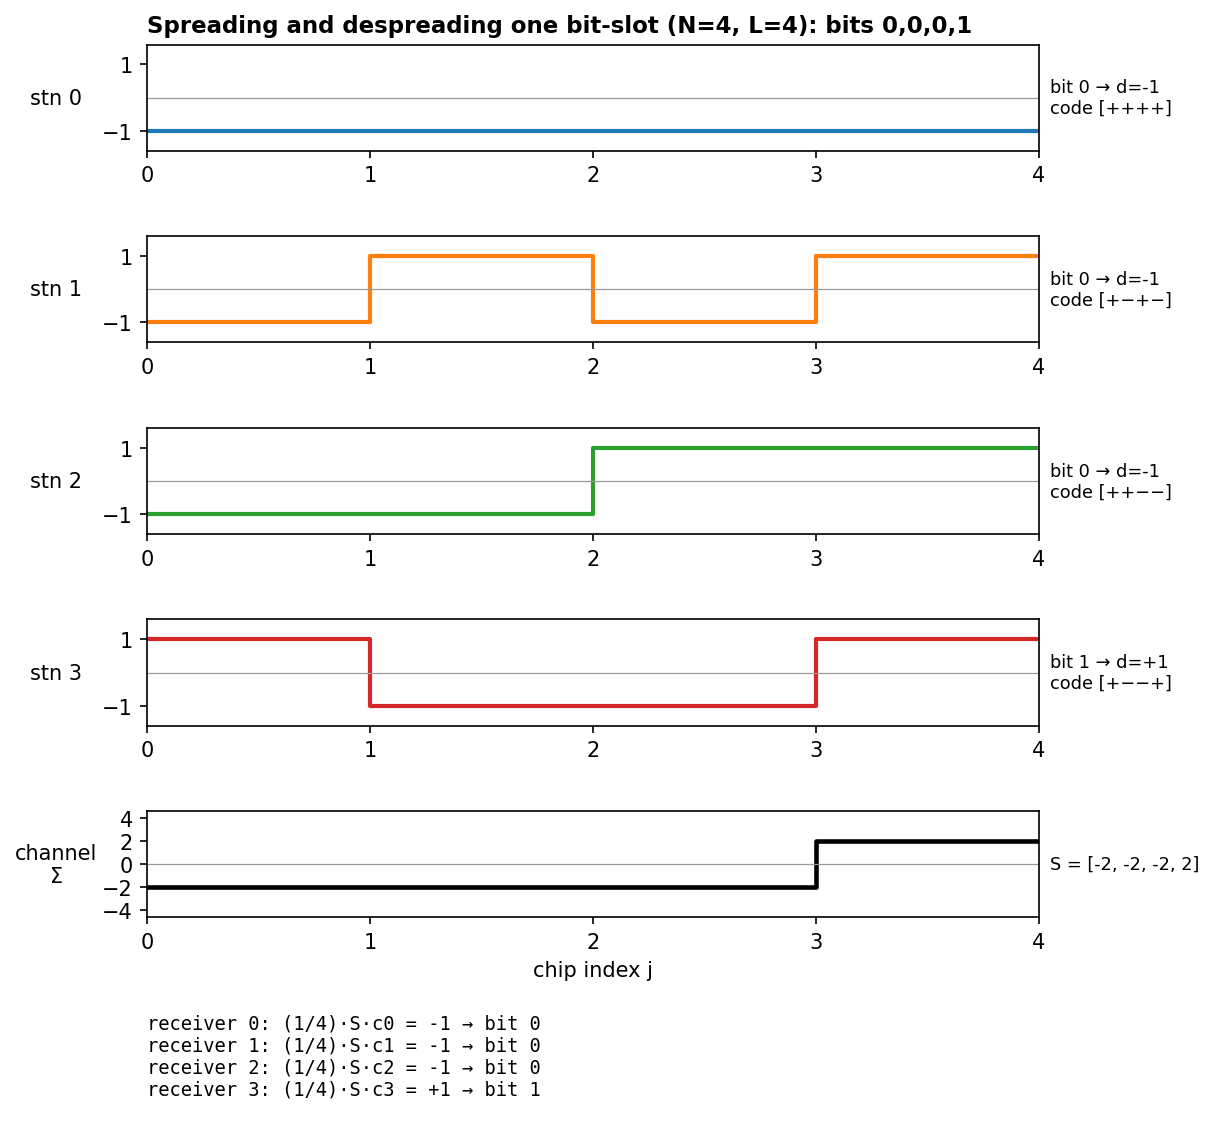
\includegraphics[width=0.82\textwidth]{figures/spreading_example.png}
\caption{Spreading and despreading in one bit-slot of the $N=4$, $L=4$ demo (slot 2 of the
trace in \S1.5). The channel carries only $S=[-2,-2,-2,+2]$, yet each receiver recovers its
own bit exactly.}
\label{fig:spread}
\end{figure}

\subsection{Performance Metrics}
\begin{itemize}[leftmargin=1.6em]
  \item \textbf{Bit error rate (BER)}: bit errors / data bits sent, counted by the server
  per slot per station. An error is any slot where a sender sent a bit and its receiver
  decoded a different symbol (the wrong bit, or ``silent'').
  \item \textbf{Exact file reconstruction}: number of receivers whose output file is
  byte-identical to their sender's input (checked by \texttt{run\_experiments.py}).
  \item \textbf{Channel efficiency}: data bits delivered per chip on the channel,
  $\dfrac{\text{data\_bits}}{\text{slots}\times L}$. With all $N$ stations busy every slot
  this equals $N/L$.
  \item \textbf{Code length $L$}: chips per bit, i.e.\ the bandwidth expansion factor
  relative to a single unspread station.
\end{itemize}

\section{Test Cases}
\begin{itemize}[leftmargin=1.6em]
  \item \textbf{TC1: Hand-checkable worked example.} $N=4$, $L=4$, messages
  \texttt{"Hi"}, \texttt{"CDMA!"}, \texttt{"Walsh"}, \texttt{"ok"}. \emph{Checking:}
  every slot of the demo trace can be verified by hand against Figure~\ref{fig:spread}; all
  four output files match (\texttt{cmp} silent); 112 bits, 0 errors.
  \item \textbf{TC2: Orthogonality of the generated codes.} \emph{Checking:}
  $W_L W_L^\top = L\,I$ for the matrix produced by the same Sylvester recursion
  (Figure~\ref{fig:walsh}, middle). This is the property every other result depends on.
  \item \textbf{TC3: Exact reconstruction for every $N$, including non-powers of two.}
  Fifteen values of $N$ from 1 to 64, including non-powers of two such as 3, 5, 6, 10, 12, 20,
  24 and 48; noiseless channel (Experiment A).
  \emph{Checking:} $0$ bit errors and \emph{every} file byte-identical in all 15 runs
  (Table~\ref{tab:expA}): 255 receivers in total, 1.29 million bits.
  \item \textbf{TC4: Unequal message lengths (silent stations).} In Experiment A, station
  $i$ sends $200+25i$ bytes, so for most of each run some senders are silent while others
  still transmit. \emph{Checking:} \texttt{silence\_errors}$=0$ (no receiver ever decoded a
  phantom bit from a silent sender) and no bits were lost from active senders.
  \item \textbf{TC5: Edge-case payloads.} $N=3$: one text file, one \emph{empty} file, and
  one 27{,}816-byte \emph{binary} file (an ELF executable). \emph{Checking:} all three outputs
  byte-identical; the empty file's receiver produced a 0-byte file; 222{,}568 bits, 0 errors.
  \item \textbf{TC6: Invalid configurations are rejected.} \texttt{N=5} with Walsh
  \texttt{L=4}. \emph{Checking:} the server exits with \emph{``Walsh codes need a
  power-of-two length $\ge$ N''}. A second \texttt{sender} registering with an id already in
  use is dropped (\emph{``duplicate SENDER 0, dropping''}) and the run completes normally.
  \item \textbf{TC7: Noise robustness matches theory.} $\sigma\in[0,4]$,
  $L=N\in\{4,\dots,64\}$ (Experiment B). \emph{Checking:} measured BER agrees with the
  analytical $Q(0.5\sqrt{L}/\sigma)$ to within sampling error at every point
  (Table~\ref{tab:expB}).
  \item \textbf{TC8: No multiple-access interference.} Fixed $L=16$, $\sigma=1.5$,
  $N=1\ldots16$ (Experiment B2). \emph{Checking:} BER is flat in $N$ (0.0896--0.0925
  against theory 0.0912). Adding users does not hurt existing ones.
  \item \textbf{TC9: Orthogonality is what makes it work.} Walsh vs.\ random $\pm1$ codes,
  $L=16$, noiseless (Experiment C). \emph{Checking:} Walsh stays at BER $=0$ while random
  codes fail from $N=4$ on (Table~\ref{tab:expC}).
  \item \textbf{TC10: Scale and liveness.} $N=64$ means 129 concurrent processes.
  \emph{Checking:} completes in 12.6\,s with exact reconstruction; no deadlock in the
  lock-step protocol across all 133 runs of the experiment suite.
\end{itemize}

\section{Results}

\subsection{Experiment A: Correctness and Scaling (Walsh, Noiseless)}
\label{sec:expA}

\begin{table}[H]
\centering
\small
\begin{tabular}{rrrrrrr}
\toprule
\textbf{N} & \textbf{L} & \textbf{Slots} & \textbf{Data bits} & \textbf{Bit errors} &
\textbf{Files exact} & \textbf{Bits/chip} \\
\midrule
1  & 1  & 1600  & 1600   & 0 & 1/1   & 1.000 \\
2  & 2  & 1800  & 3400   & 0 & 2/2   & 0.944 \\
3  & 4  & 2000  & 5400   & 0 & 3/3   & 0.675 \\
4  & 4  & 2200  & 7600   & 0 & 4/4   & 0.864 \\
5  & 8  & 2400  & 10000  & 0 & 5/5   & 0.521 \\
6  & 8  & 2600  & 12600  & 0 & 6/6   & 0.606 \\
8  & 8  & 3000  & 18400  & 0 & 8/8   & 0.767 \\
10 & 16 & 3400  & 25000  & 0 & 10/10 & 0.460 \\
12 & 16 & 3800  & 32400  & 0 & 12/12 & 0.533 \\
16 & 16 & 4600  & 49600  & 0 & 16/16 & 0.674 \\
20 & 32 & 5400  & 70000  & 0 & 20/20 & 0.405 \\
24 & 32 & 6200  & 93600  & 0 & 24/24 & 0.472 \\
32 & 32 & 7800  & 150400 & 0 & 32/32 & 0.603 \\
48 & 64 & 11000 & 302400 & 0 & 48/48 & 0.430 \\
64 & 64 & 14200 & 505600 & 0 & 64/64 & 0.556 \\
\bottomrule
\end{tabular}
\caption{Experiment A: Walsh codes, $\sigma=0$, station $i$ sends $200+25i$ bytes of text.
Every receiver reconstructs its file exactly.}
\label{tab:expA}
\end{table}

\begin{figure}[H]
\centering
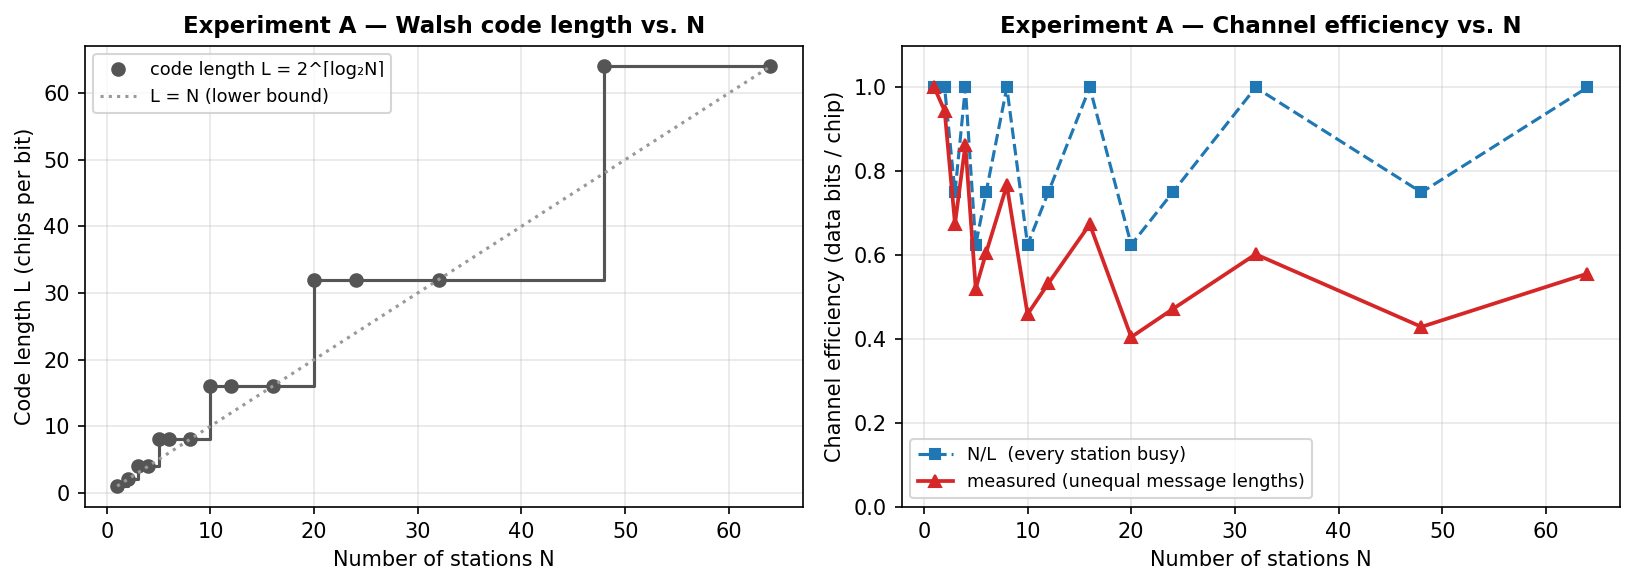
\includegraphics[width=\textwidth]{figures/expA_efficiency.png}
\caption{Left: Walsh code length grows in powers of two. Right: channel efficiency.
$N/L$ is the ceiling with every station busy; the measured value is lower because
stations with shorter messages fall silent while the longest one finishes.}
\label{fig:expA}
\end{figure}

\begin{figure}[H]
\centering
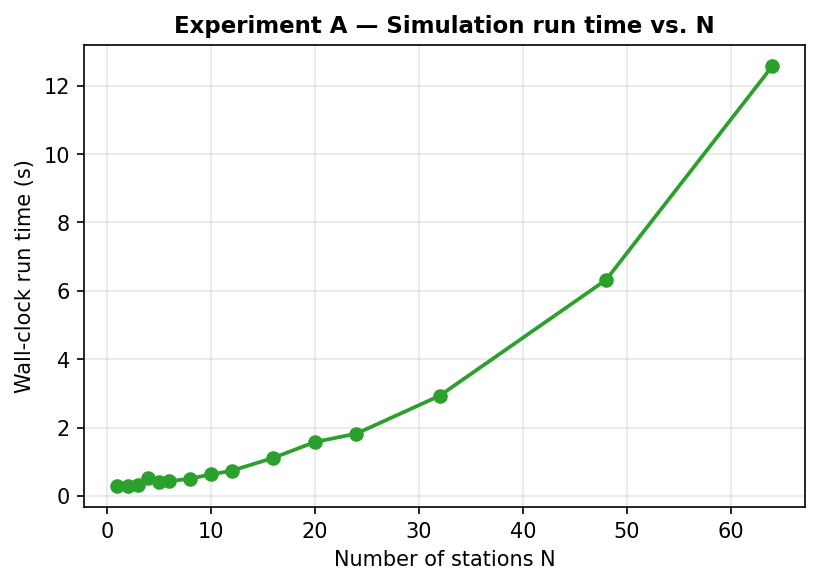
\includegraphics[width=0.7\textwidth]{figures/expA_runtime.png}
\caption{Wall-clock time of each Experiment A run (simulation cost, not a protocol metric).}
\end{figure}

\subsection{Experiment B: BER Under Channel Noise}
\label{sec:expB}
Each station sends 500 random bytes (4000 bits); $N=L$ (every code in use); Gaussian noise
of standard deviation $\sigma$ is added to every chip.

\begin{table}[H]
\centering
\small
\begin{tabular}{r ll ll ll ll ll}
\toprule
& \multicolumn{2}{c}{\textbf{L = 4}} & \multicolumn{2}{c}{\textbf{L = 8}} &
  \multicolumn{2}{c}{\textbf{L = 16}} & \multicolumn{2}{c}{\textbf{L = 32}} &
  \multicolumn{2}{c}{\textbf{L = 64}} \\
\cmidrule(lr){2-3}\cmidrule(lr){4-5}\cmidrule(lr){6-7}\cmidrule(lr){8-9}\cmidrule(lr){10-11}
$\sigma$ & meas. & theory & meas. & theory & meas. & theory & meas. & theory & meas. & theory \\
\midrule
0.00 & 0      & 0      & 0      & 0      & 0       & 0       & 0       & 0       & 0       & 0 \\
0.25 & 6.3e-5 & 3.2e-5 & 0      & 8e-9   & 0       & 0       & 0       & 0       & 0       & 0 \\
0.50 & 0.0233 & 0.0228 & 0.0019 & 0.0023 & 1.6e-5  & 3.2e-5  & 0       & 8e-9    & 0       & 0 \\
0.75 & 0.0943 & 0.0912 & 0.0294 & 0.0297 & 0.0042  & 0.0038  & 4.7e-5  & 8.1e-5  & 0       & 5e-8 \\
1.00 & 0.1600 & 0.1587 & 0.0767 & 0.0787 & 0.0224  & 0.0228  & 0.0024  & 0.0023  & 3.5e-5  & 3.2e-5 \\
1.25 & 0.2134 & 0.2119 & 0.1278 & 0.1290 & 0.0550  & 0.0548  & 0.0114  & 0.0118  & 6.9e-4  & 6.9e-4 \\
1.50 & 0.2526 & 0.2525 & 0.1743 & 0.1729 & 0.0905  & 0.0912  & 0.0305  & 0.0297  & 0.0037  & 0.0038 \\
2.00 & 0.3095 & 0.3085 & 0.2358 & 0.2398 & 0.1576  & 0.1587  & 0.0776  & 0.0787  & 0.0232  & 0.0228 \\
2.50 & 0.3416 & 0.3446 & 0.2815 & 0.2858 & 0.2125  & 0.2119  & 0.1291  & 0.1290  & 0.0560  & 0.0548 \\
3.00 & 0.3695 & 0.3694 & 0.3185 & 0.3187 & 0.2520  & 0.2525  & 0.1719  & 0.1729  & 0.0920  & 0.0912 \\
4.00 & 0.4038 & 0.4013 & 0.3585 & 0.3618 & 0.3080  & 0.3085  & 0.2403  & 0.2398  & 0.1597  & 0.1587 \\
\bottomrule
\end{tabular}
\caption{Experiment B: measured BER vs.\ the analytical $Q(0.5\sqrt{L}/\sigma)$ (theory values below $10^{-15}$ shown as 0). Sample
sizes are $16{,}000$ ($L=4$) to $256{,}000$ ($L=64$) bits per point, so the smallest
non-zero BER measurable is $\approx 4\times10^{-6}$ to $6\times10^{-5}$.}
\label{tab:expB}
\end{table}

\begin{figure}[H]
\centering
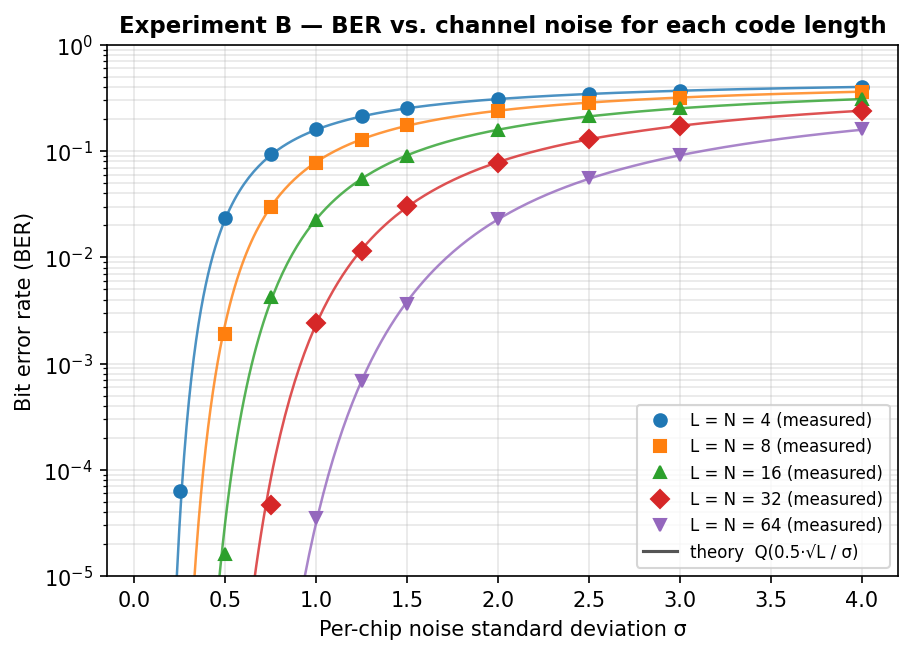
\includegraphics[width=0.85\textwidth]{figures/expB_ber_sigma.png}
\caption{BER vs.\ per-chip noise for each code length (markers: measured; lines: theory).
Points with zero errors cannot be drawn on the log axis.}
\label{fig:expB}
\end{figure}

\begin{figure}[H]
\centering
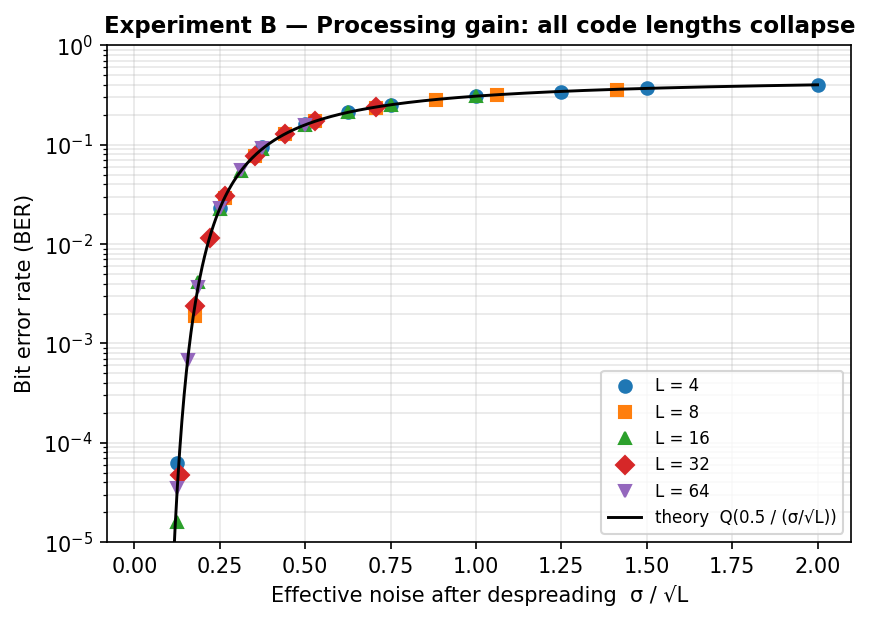
\includegraphics[width=0.82\textwidth]{figures/expB_processing_gain.png}
\caption{The same data re-plotted against the post-despreading noise $\sigma/\sqrt{L}$:
all five code lengths fall on one curve.}
\label{fig:pg}
\end{figure}

\paragraph{Experiment B2: BER vs.\ number of active stations.} $L=16$, $\sigma=1.5$, 1000
random bytes per station.

\begin{table}[H]
\centering
\small
\begin{tabular}{rrrr}
\toprule
\textbf{N} & \textbf{Data bits} & \textbf{Bit errors} & \textbf{BER} \\
\midrule
1  & 8000   & 717   & 0.0896 \\
2  & 16000  & 1443  & 0.0902 \\
4  & 32000  & 2960  & 0.0925 \\
6  & 48000  & 4320  & 0.0900 \\
8  & 64000  & 5833  & 0.0911 \\
10 & 80000  & 7327  & 0.0916 \\
12 & 96000  & 8877  & 0.0925 \\
14 & 112000 & 10210 & 0.0912 \\
16 & 128000 & 11779 & 0.0920 \\
\bottomrule
\end{tabular}
\caption{Experiment B2: BER does not depend on $N$ (theory: $Q(0.5\cdot4/1.5) = 0.0912$).}
\label{tab:expB2}
\end{table}

\begin{figure}[H]
\centering
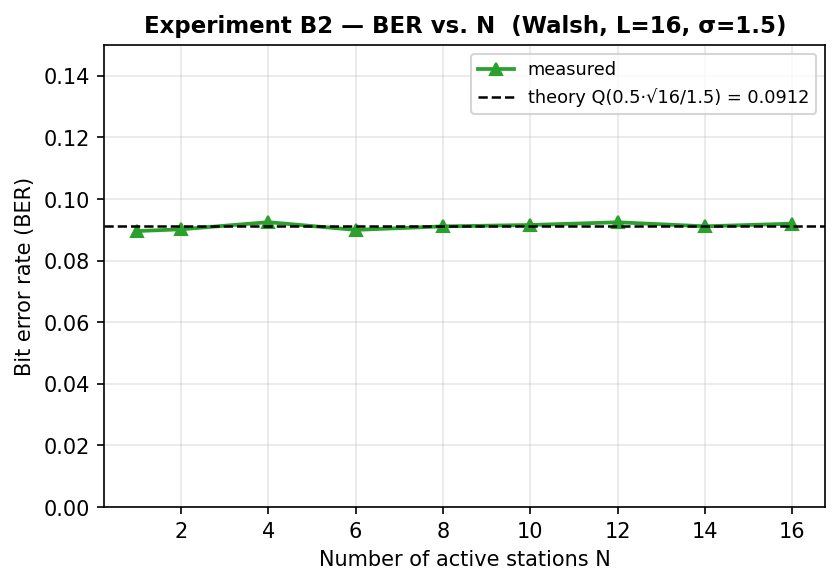
\includegraphics[width=0.72\textwidth]{figures/expB2_ber_vs_n.png}
\caption{BER vs.\ number of simultaneously transmitting stations at fixed $L$ and $\sigma$.}
\end{figure}

\subsection{Experiment C: Walsh vs.\ Random Codes}
\label{sec:expC}
$L=16$ for both code families, $\sigma=0$ (no noise at all, so every error is caused by
interference between stations), 250 random bytes per station. Random codes are averaged
over 5 seeds.

\begin{table}[H]
\centering
\small
\begin{tabular}{rrrrr}
\toprule
& \multicolumn{2}{c}{\textbf{Walsh}} & \multicolumn{2}{c}{\textbf{Random $\pm1$ (5 seeds)}} \\
\cmidrule(lr){2-3}\cmidrule(lr){4-5}
\textbf{N} & \textbf{BER} & \textbf{Files exact} & \textbf{BER mean [min, max]} & \textbf{Files exact (mean)} \\
\midrule
1  & 0 & 1/1   & 0 \; [0, 0]                 & 1.0 / 1 \\
2  & 0 & 2/2   & 0 \; [0, 0]                 & 2.0 / 2 \\
4  & 0 & 4/4   & 0.152 \; [0.060, 0.260]     & 1.2 / 4 \\
6  & 0 & 6/6   & 0.204 \; [0.116, 0.281]     & 0.4 / 6 \\
8  & 0 & 8/8   & 0.242 \; [0.197, 0.300]     & 0 / 8 \\
10 & 0 & 10/10 & 0.252 \; [0.214, 0.271]     & 0 / 10 \\
12 & 0 & 12/12 & 0.299 \; [0.260, 0.334]     & 0 / 12 \\
14 & 0 & 14/14 & 0.337 \; [0.326, 0.350]     & 0 / 14 \\
16 & 0 & 16/16 & 0.338 \; [0.311, 0.355]     & 0 / 16 \\
\bottomrule
\end{tabular}
\caption{Experiment C: noiseless channel, same code length, different code families.}
\label{tab:expC}
\end{table}

\begin{figure}[H]
\centering
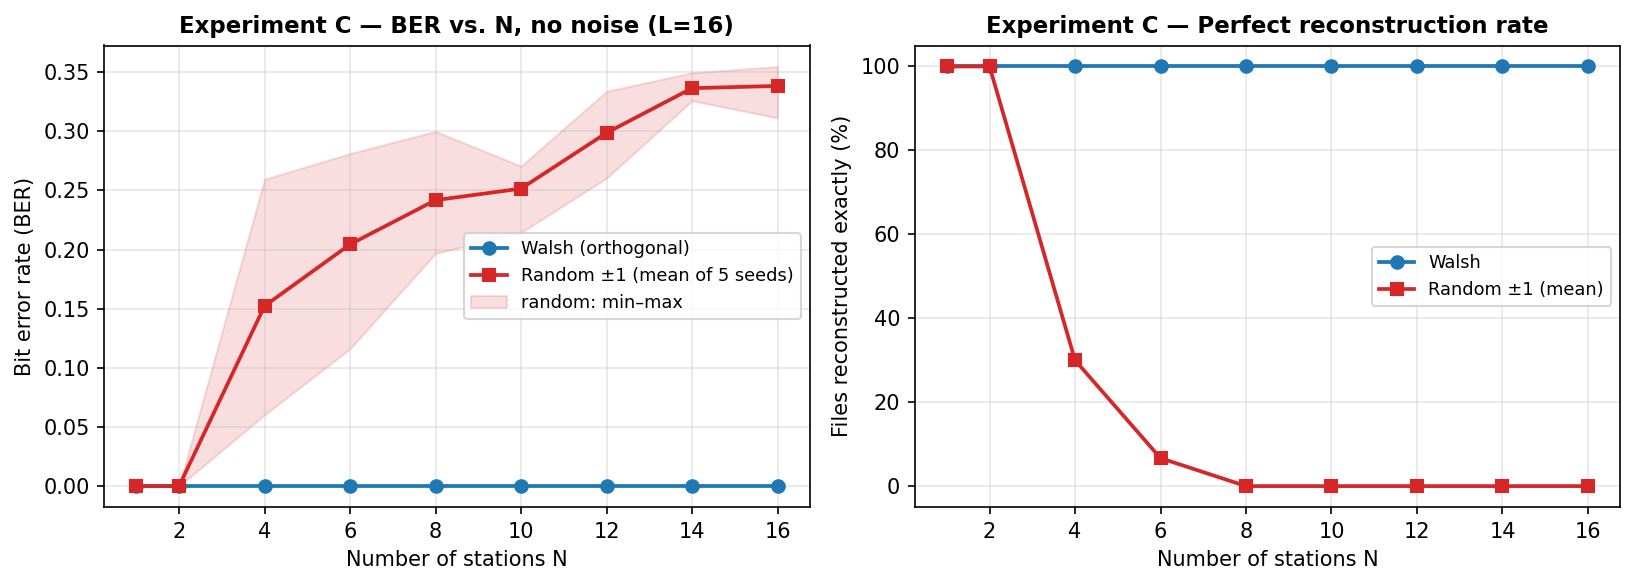
\includegraphics[width=\textwidth]{figures/expC_walsh_vs_random.png}
\caption{Left: BER vs.\ $N$ (shaded: min--max over 5 random-code seeds). Right: percentage of
stations whose file was reconstructed exactly.}
\label{fig:expC}
\end{figure}

\section{Analysis}

\subsection{Why reconstruction is perfect (Experiment A)}
Every one of the 255 receivers across 15 runs, from $N=1$ to $N=64$, reproduced its file
byte-for-byte, with zero silence errors despite stations finishing at different times. This
is not luck or a forgiving threshold; it follows directly from the algebra in \S1.2. In a
noiseless channel the composite signal is a vector of small integers, the despreading
product $S\cdot c_i$ is computed exactly, and the cross terms $c_k\cdot c_i$ are exactly
zero for $k\neq i$. So $v_i$ is exactly $+1$, $-1$ or $0$, never anything in between, and
the $\pm0.5$ thresholds have a full margin of $0.5$ on every side. The worked example in
Figure~\ref{fig:spread} shows the effect concretely: the channel signal
$[-2,-2,-2,+2]$ looks nothing like any individual station's waveform, yet each of the four
dot products lands exactly on $\pm1$.

\subsection{The cost of CDMA: bandwidth expansion}
Perfect separation is paid for in chips. Each bit occupies $L$ chips, so a single station's
bit rate is $1/L$ of the raw channel chip rate, and the channel as a whole delivers at most
$N/L$ bits per chip. Two effects pull the measured efficiency below 1:
\begin{itemize}[leftmargin=1.6em]
  \item \textbf{Power-of-two rounding.} Walsh codes exist only for $L=2^k$, so $N$ just
  above a power of two wastes almost half the code space. At $N=5$ the system must use
  $L=8$ (ceiling $5/8=0.625$); at $N=20$, $L=32$ (ceiling 0.625); at $N=48$, $L=64$
  (ceiling 0.75). The ceiling returns to $1$ only at $N=2^k$ (Figure~\ref{fig:expA}).
  \item \textbf{Idle codes.} A silent station still ``owns'' its code; nobody else can use
  that dimension. In Experiment A message lengths differ by up to $25(N-1)$ bytes, so
  towards the end of each run most codes carry zeros. For example, at $N=64$ the measured
  efficiency is 0.556 against a ceiling of 1.0.
\end{itemize}
With $N=L$ and all stations busy, synchronous Walsh CDMA delivers exactly one bit per chip,
the same as ideal TDMA with $N$ slots. Both schemes divide an $L$-dimensional signal space
into $N$ orthogonal pieces; TDMA uses time-slot indicator vectors as its ``codes'' and CDMA
uses Walsh rows. The difference shows up in the next two subsections, under noise and when
users are not coordinated in time.

\subsection{Processing gain under noise (Experiment B)}
Measured BER tracks $Q(0.5\sqrt{L}/\sigma)$ to within sampling error at all 55 points
(Table~\ref{tab:expB}). For example, at $L=32$, $\sigma=2$ the measured value is 0.0776
against a predicted 0.0787. The longer the code, the more noise is tolerated. At $\sigma=1$
(noise per chip as large as the signal itself) BER falls from 0.160 at $L=4$ to
$3.5\times10^{-5}$ at $L=64$. The reason is the averaging in despreading. The wanted signal
adds coherently over $L$ chips (amplitude $\times L$) while independent noise adds
incoherently (amplitude $\times\sqrt{L}$), so the effective noise is $\sigma/\sqrt{L}$.
Figure~\ref{fig:pg} confirms this: plotted against $\sigma/\sqrt{L}$, all five code lengths
collapse onto a single curve. Every doubling of $L$ buys
$10\log_{10}2 \approx 3$\,dB of noise immunity, the classical spread-spectrum processing
gain.

\paragraph{BER is independent of $N$ (Experiment B2).} With $L=16$ and $\sigma=1.5$, BER
stays within $0.0896$--$0.0925$ for $N=1$ through $16$, scattered around the predicted
$0.0912$ with no trend (Table~\ref{tab:expB2}). Adding a sixteenth simultaneous transmitter
degrades the first one no more than having it alone on the channel. This is the
experimental form of ``MAI $=0$'': the noise floor, not the number of users, limits
reliability.

\subsection{Why orthogonality matters (Experiment C)}
Random $\pm1$ codes of the same length look superficially similar: each is a ``unique code
word'', and with no noise at all they still fail badly. BER rises to 0.15 at $N=4$ and
0.34 at $N=16$, and from $N=8$ onwards not a single file was reconstructed in any of the 25 runs.
The cause is the MAI term of \S1.2. For random codes $c_k\cdot c_i\neq 0$, so receiver $i$
sees
$v_i = d_i + \tfrac{1}{L}\sum_{k\neq i} d_k (c_k\cdot c_i)$, and the interference has
variance $\approx (N-1)/L$. It grows with every added user until it routinely pushes $v_i$
across a threshold. The right-hand matrix of Figure~\ref{fig:walsh} shows these non-zero
cross-correlations for $L=8$.

The perfect result at $N=2$ for random codes is not a contradiction. With one interferer,
an error needs $|c_1\cdot c_2|\ge 8$ when $L=16$, so that $v$ is pushed onto or past the
$\pm0.5$ thresholds. For two random 16-chip codes this happens with probability
$2\sum_{m=0}^{4}\binom{16}{m}/2^{16}\approx 7.7\%$, and none of the five seeds drew such a
pair. With three or more users the interference terms add, and errors appear immediately.
Walsh codes remove this randomness altogether: $c_k\cdot c_i = 0$ by construction, so
there are \emph{no} unlucky code assignments.

\subsection{A design trade-off: the three-level decision}
The silence level ($d=0$) lets stations send variable-length messages with no length header,
but it halves the decision margin. A transmitted $+1$ is lost as soon as
$v < 0.5$, not $v < 0$, which is why the theory is $Q(0.5\sqrt{L}/\sigma)$ instead of the
binary $Q(\sqrt{L}/\sigma)$, a $6$\,dB penalty. It also makes the error mode worse. A
$\pm1$ misread as ``silent'' \emph{drops} a bit, shifting every later bit of that file by
one position, so the file is ruined rather than having a single flipped bit. In
Experiment B a single error is enough to spoil a file: at $L=64$, $\sigma=1.0$ (BER
$3.5\times10^{-5}$) 55 of 64 files survive, but at $\sigma=1.25$ (BER $6.9\times10^{-4}$, about
three errors per 4000-bit file) only 6 of 64 do. In the noiseless Walsh case, the case the assignment asks for, the margin
is never needed and reconstruction is exact.

\subsection{Known limitations}
\begin{itemize}[leftmargin=1.6em]
  \item \textbf{Perfect chip synchronisation is assumed.} The lock-step server aligns all
  senders' chips exactly. Real uplinks are asynchronous, and shifted Walsh codes are
  \emph{not} orthogonal. Practical systems therefore use Walsh codes on the synchronous
  downlink and long pseudo-noise codes on the uplink.
  \item \textbf{Equal received power.} Every sender contributes amplitude $\pm1$. With
  unequal powers and non-orthogonal codes, a strong nearby station would swamp a weak one
  (the near--far problem), which real CDMA counters with power control.
  \item \textbf{Text protocol overhead.} Chips are sent as ASCII integers over TCP. This is
  fine for a simulation, but it dominates the run time at large $N$ (12.6\,s for $N=64$).
\end{itemize}

\section{Comments}

\paragraph{Evaluation of the Lab Assignment.} This assignment completes a progression. In
Assignment 3, simultaneous transmission was the failure case that every protocol tried to
avoid, while here it is the normal mode of operation. Seeing $[-2,-2,-2,+2]$ on the
channel and watching four independent processes each pull a different, correct bit out of
it makes the linear algebra behind CDMA tangible in a way the textbook equations alone do
not. Reusing the server + independent-process design from Assignment 3 also kept the focus
on the coding scheme rather than on new plumbing.

\paragraph{Difficulty and Learning Outcomes.} The core of the assignment, spreading with a
Walsh row and despreading with a dot product, is short; the noiseless Walsh case cannot fail
once the codes are orthogonal and aligned. It was therefore less difficult than
Assignment~3. The more instructive work was in deciding \emph{what to test against}. Without
the noise and random-code experiments, ``all files match'' would only show that the
arithmetic is correct, not \emph{why} Walsh codes are required, or what the $L$-fold
bandwidth cost buys in return (the processing gain of Experiment B). Matching the measured
BER curves to $Q(0.5\sqrt{L}/\sigma)$ at every point was also a strong end-to-end check that
the noise model, the despreading and the error accounting are all correct.

\paragraph{Suggested Improvements.} (1) Send a short length header (or use a fixed frame
length) so receivers can use a plain sign decision, recovering the 6\,dB lost to the silence
level and turning a lost bit into a flipped bit. (2) Add a chip-offset option to the server
to show how quickly Walsh orthogonality breaks down without synchronisation. (3) Assign codes
dynamically, giving a code to a station only while it has data, so that the idle-code waste
seen in Experiment A could be reclaimed. This would combine the CDMA physical layer with the
MAC-layer ideas of Assignment 3.

\end{document}
